A variable can be mapped to a channel. Creating a variable $x$ and initializing it with the value $0$ ( int x = 0;) is mapped to creating a new channel x and initialize the processes Zero with the channel x
as shown in \refFig{tra_var}. The wide hat refers to creating a new channel.
\begin{figure}[H]%
\centering
\subcaptionbox{ABC code.}{\fbox{$(\ \widehat{}\ \text{x}\ )\ (\ \text{Zero}(\text{x})\ )$}}%
\hspace{1em}%
\subcaptionbox{visualization.}{\fbox{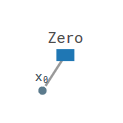
\includegraphics[]{./images/transformational_semantics_of_oz/var.png}}}%
\caption{Variable as a channel.}
\label{tra_var}%
\end{figure}

Thus, we map the state variables $self, cv, tv, message$ of \refFig{oz_vm_reference_name} to \picalc{} channels $self, cv, tv, message$ as shown in \refFig{tra_var2}

\begin{figure}[H]
\centering
\fbox{  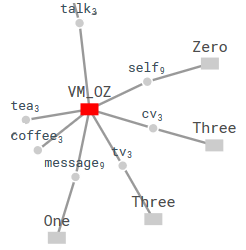
\includegraphics[width=.5\linewidth]{./images/transformational_semantics_of_oz/vm_OZ.png}}
\caption{VM as a \picalc{} process VM\_OZ.}
\label{tra_var2}
\end{figure}